\documentclass[sigconf,natbib=false, language=english]{acmart}

% Ne dodajaj hyperref (acmart ga že naloži)
\settopmatter{printccs=false, printacmref=false}


% BEGIN BIBLIOGRAPHY CONFIGURATION
% --------------------------------------------- %

\usepackage[datamodel=acmdatamodel, style=acmnumeric, backend=biber]{biblatex}
\addbibresource{refs.bib}
%\renewcommand*{\bibfont}{\footnotesize}

% --------------------------------------------- %
% END BIBLIOGRAPHY CONFIGURATION

\AtBeginDocument{%
  \providecommand\BibTeX{{%
    Bib\TeX}}}

\renewcommand\footnotetextcopyrightpermission[1]{}
\setcopyright{rightsretained}
\copyrightyear{2025}
\acmDOI{10.70314/is.2025.sikdd.30}
\acmISBN{}
\acmConference[Information Society 2025]{Information Society 2025: 28th international multiconference}{6--10 October 2025}{Ljubljana, Slovenia}
\settopmatter{printccs=false, printacmref=false}

\geometry{a4paper}
\begin{document}


\title[Ski Jumping Simulation]{Predicting Ski Jumps Using State-Space Model}

\author{Neca Camlek}
\authornote{Both authors contributed equally to this research.}
\affiliation{%
  \institution{Univerza v Ljubljani}
  \city{Ljubljana}\country{Slovenia}}
  
\author{Živa Hegler}
\authornotemark[1] 
\affiliation{%
  \institution{Univerza v Ljubljani}
  \city{Ljubljana}\country{Slovenia}}
  
\author{Jakob Jelenčič}
\affiliation{%
  \institution{Jožef Stefan Institute}
  \city{Ljubljana}\country{Slovenia}}
\email{jakob.jelencic@ijs.si}

\author{Marko Grobelnik}
\affiliation{%
  \institution{Jožef Stefan Institute}
  \city{Ljubljana}\country{Slovenia}}
\email{marko.grobelnik@ijs.si}

\author{Dunja Mladenić}
\affiliation{%
  \institution{Jožef Stefan Institute}
  \city{Ljubljana}\country{Slovenia}}
\email{dunja.mladenic@ijs.si}


\renewcommand{\shortauthors}{Ž. Hegler, N. Camlek et al.}


\begin{abstract}

Ski jumping performance is shaped by both athlete technique and environmental conditions, with factors such as wind speed, wind direction, and ski orientation playing a critical role in determining jump trajectories. Accurate modeling of these trajectories is challenging due to dynamic and time-dependent nature of the data. In this work, we introduce a dataset of measured ski jumps and present a state-space modeling framework that captures the evolution of jumps under varying conditions. The model parameters are estimated using a ridge regression approach, 
enabling us to predict trajectories from initial states and wind sensor inputs. 
We evaluated the predictive performance of the model through leave-one-out cross-validation and analyzed its stability, showing that the approach can predict realistic trajectories with reasonable accuracy. To complement the modeling results, we developed an interactive web application that allows users to explore both recorded and simulated jumps, adjust environmental factors, and visualize their effects through animations. Together, the dataset, modeling framework, and the web application offer a foundation for further research in ski jump analysis and provide an accessible tool for exploring the influence of external conditions on performance.

\end{abstract}

\keywords{datasets, state-space model, ski jumping, simulations, least squares}

%%\received{20 August 2025}
%%\received[revised]{13 September 2025}
%%\received[accepted]{15 September 2025}

%% This command processes the author and affiliation and title
%% information and builds the first part of the formatted document.
\maketitle

\section{Introduction}
%kaj delava
%kaj je problem in kako ga drugi rešujejo
%piševa na kakšne načine drugi lahko to delajo, kakšne opcije obstajajo


Ski jumping is a sport strongly influenced by both athletic technique and environmental conditions.
Factors such as wind speed, wind direction, and different ski angles affect the trajectory and final distance of a jump, making accurate prediction a challenging problem. 
While statistical models and simulations have been applied in sports research for some time, many approaches simplify the problem and do not fully capture the dynamic evolution of the jump over time \cite{SkiJumping_Book, fang2020trajectory, schwinn2022xlength, zecha2018convolutional}.

Recent advances in machine learning have introduced methods capable of modeling temporal systems with greater fidelity. In particular, state-space models provide a mathematical framework for representing hidden internal states that evolve over time in response to external input. This makes them well-suited for modeling ski jumps, where environmental factors determine performance \cite{SSM_YouTube}.

In this paper, we present a ski jump dataset together with a 
state-space model trained to predict jump trajectories based on 
changing environmental conditions. 
The model is estimated using a least squares approach and demonstrates 
how inputs such as wind and ramp adjustments influence the resulting 
jump. Beyond the modeling framework, we also developed an application 
that allows general users to interact with the data, run simulations, 
and visualize jump trajectories through animations. 

The main contributions of this paper are threefold. 
First, we propose a novel approach for modeling ski jump trajectories 
based on a state-space formulation and ridge regression. 
Second, we develop and evaluate a trained state-space model capable 
of predicting ski jump trajectories under changing environmental 
conditions. Third, we present an interactive web application for 
exploratory data analysis, jump simulation, and visualization. 
Beyond these methodological contributions, accurate prediction of ski 
jumps can improve athlete safety by anticipating risky conditions, 
support planning of hill design or enlargement, and contribute to 
fairer competitions through a better understanding of environmental 
effects.

The remainder of the paper is as follows. Section~\ref{sec:related} reviews
related work and then section~\ref{sec:data} presents the handling of received data. Next, the proposed methodology is described in Section~\ref{sec:method}. 
The project results are presented in Section~\ref{sec:results}. We discuss the results in Section~\ref{sec:discussion} and conclude the paper in Section~\ref{sec:conclusion}.

\section{Related Work}\label{sec:related}

Several approaches have been explored for modeling and predicting ski jump
trajectories, ranging from physics-based simulations to data-driven methods.

Fang et al. \cite{fang2020trajectory} proposed a state-space approach for
reconstructing ski jump trajectories from wearable inertial sensors, using an
Extended Rauch-Tung-Striebel (RTS) smoother with state constraints to estimate
position and velocity during flight. While their focus was on reconstruction
from sensor data rather than prediction from environmental inputs, their use of
a state-space formulation for capturing jump dynamics is closely related to our
approach.

Schwinn et al. \cite{schwinn2022xlength} introduced \textit{xLength}, a
deep learning framework for predicting the expected jump length shortly after
take-off. Using a dataset of 2523 jumps from 205 athletes across five venues,
they evaluated fully connected networks, CNNs, LSTMs, and ResNet architectures,
achieving a mean absolute error of 5.3~m when generalizing to new athletes.
Their work highlights the potential of sensor-based data for jump length
prediction, though it focuses on length estimation from early flight data rather
than full trajectory modeling under varying wind conditions.

Zecha et al. \cite{zecha2018convolutional} presented a convolutional
sequence-to-sequence model for predicting multimodal jump dynamics, including
trajectory and forces, from athlete pose estimates. This approach demonstrates
the use of temporal deep learning models for capturing sequential jump dynamics,
but relies on video-based pose input rather than direct environmental sensor
data.

In contrast to these works, our approach uses a linear state-space model
estimated via ridge regression, which offers greater interpretability and does
not require large datasets or deep learning infrastructure. We explicitly
incorporate wind sensor measurements as control inputs, allowing the model to
simulate how changing environmental conditions affect the full jump trajectory.

\section{Approach to Modeling}\label{sec:data}
This section describes the handling of data, focusing on state-space models and our data processing.

\begin{figure}[h]
  \centering
  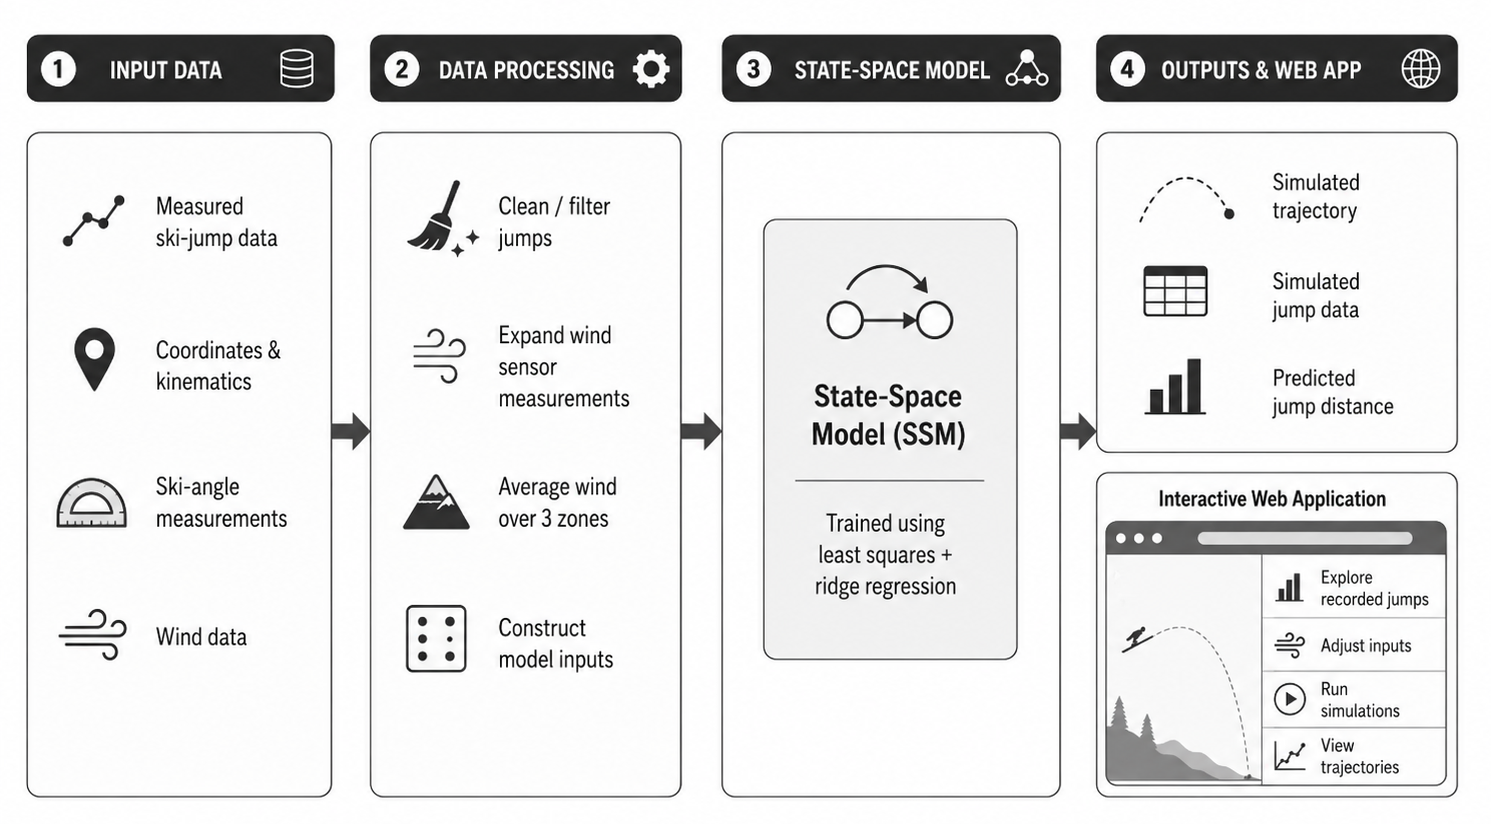
\includegraphics[width=\linewidth]{architecture.png}
  \caption{Architecture of the paper}
  \Description{A visual representation of the paper architecture }
  \label{fig:planica}
\end{figure}

\subsection{State-Space Model}\label{subsec:ssm}
State-Space Models (SSMs) are a family of machine learning algorithms designed to capture and predict the behavior of dynamic systems by describing how their inner states change over time.  
Instead of only looking at past inputs and outputs, SSMs explicitly model the underlying dynamics, making them well-suited for sequential data. In state-space modeling, 
the objective is to identify the minimal set of system variables required to completely describe the system. These fundamental variables are referred to as the state variables. 
At any given time, the state of the system can be represented by a state vector, 
whose components correspond to the values of the respective state variables. 
SSMs are designed to predict both the manner in which inputs are reflected in the system's outputs and the evolution of a system's internal state over time and in response to specific inputs \cite{aoki1990state}. 

\subsection{Least squares method}

The least squares method is a regression technique that is used to determine the line that best fits a given set of data. It minimizes the sum of the squared differences between the observed data and the corresponding values implied by the regression function. Each data point reflects the relationship between a known independent variable and an unknown dependent variable \cite{Plestenjak_NUM}. 

To enhance the model, we incorporated ridge regression (L2 regularization), which helps to reduce overfitting during model training \cite{vanWieringen2015ridge}. 

\subsection{Data Processing}\label{sec:processing}

%vse o podatkih: kakšne podatke sva dobili in kje sva jih dobili, kaj je blo v njih, 
%kako jih je blo treba spremenit lahko tko po korakih kaj je blo treba spreminjat, 
%da so bli za uporabo, lahko tko po korakih: naprej je blo treba to in pol to...

For our project, we used $223$ CSV files, each containing the data of a jump, measured on the flying hill of Gorišek brothers in Planica, Slovenia. 
Each contains 17 columns (\texttt{'Position'}, \texttt{'Height above ground'}, \texttt{'Time'}, \texttt{'X'}, \texttt{'Y'}, \texttt{'Z'}, 
\texttt{'Opening Angle'}, \\ \texttt{'Stalling Angle Left'}, \texttt{'Stalling Angle Right'}, 
\texttt{'Roll Angle Left'}, \texttt{'Roll Angle Right'}, \texttt{'Yaw Angle Left'}, \texttt{'Yaw Angle Right'}, 
\texttt{'Speed hor.'}, \texttt{'Speed vert.'}, \texttt{'Speed \\ resulting'},
\texttt{'WindTime|WindName|WindSpeed|Wind...'}) and the number of rows corresponding to the length of the jump. Data are recorded for every meter
of air distance from the take-off point.

The data required some pre-processing before it could be used for training the model.
%The column Time was written using the format: \texttt{0001-01-01T00:00:00.0000000+01:00}. Here, 
%\texttt{0001-01-01} means the date (January first in the year one), which is a place holder date, so we removed it.
%The \texttt{+01:00} at the end indicates the time zone, which we also removed.
%The remaining part \texttt{00:00:00.0000000} indicates the jump time in hours, minutes, seconds, and milliseconds.
%We converted this to a numerical value in seconds which was then used as the time variable in the model.
\\ The column \texttt{WindTime|WindName|WindSpeed|...} combined multiple attributes separated by '\texttt{|}'. Data from 12 sensors, each measuring six wind characteristics, were expanded into $12 \times 6 = 72$ columns, one per sensor–feature pair (\texttt{sensor\_feature}).
%\\ The column \texttt{WindTime|WindName|WindSpeed|Wind...} contained multiple pieces of information separated by '\texttt{|}'.
%Wind was recorded on 12 sensors placed along the hill, each measuring one of the seven wind characteristics in the order represented in the column name. To keep all the data and not multiply the time stamps, we split this column into $12 \times 6 = 72$ columns, each representing one of the wind features for one of the sensors (\texttt{sensor\_feature}).

%I THINK DA BI BLO DOBR DA TUD ZA KOTE DODAVA NEKO SLIKO
\begin{description}
    \item[Position] - air distance from the take-off point in meters. Begins with a negative value, which represents the distance from the starting point to the take-off point. In ski jumping, the starting point is adjusted according to the wind conditions, so this value is not constant.
    \item[Height above ground] - height above ground in meters.
    \item[Time] - time of the jump in seconds from the start of the jump.
    \item[X, Y, Z] - coordinates of the jumper in a 3D space in meters. The X axis is aligned with the hill direction,
    the Y axis is across the hill, and the Z axis is vertical. The take-off point is $(0,0,0)$ as shown in Figure~\ref{fig:planica}
    \item[Opening Angle] - angle between the skis in degrees.
    \item[Stalling Angle Left, Stalling Angle Right] - angle between the chord line of the left/right ski and the horizontal plane in degrees.
    \item[Roll Angle Left, Roll Angle Right] - angle of the left/right ski around its longitudinal axis relative to the horizontal plane in degrees.
    \item[Yaw Angle Left, Yaw Angle Right] - angle between the \\ left/right ski and the horizontal plane in degrees. 
    \\ (angles are shown in Figure~\ref{fig:koti})
    \item[Speed hor., Speed vert., Speed resulting] - horizontal, vertical, and the resulting speed of the athlete in km/h \cite{virmavirta2019aerodynamics}. 
\end{description}

\begin{figure}[h]
  \centering
  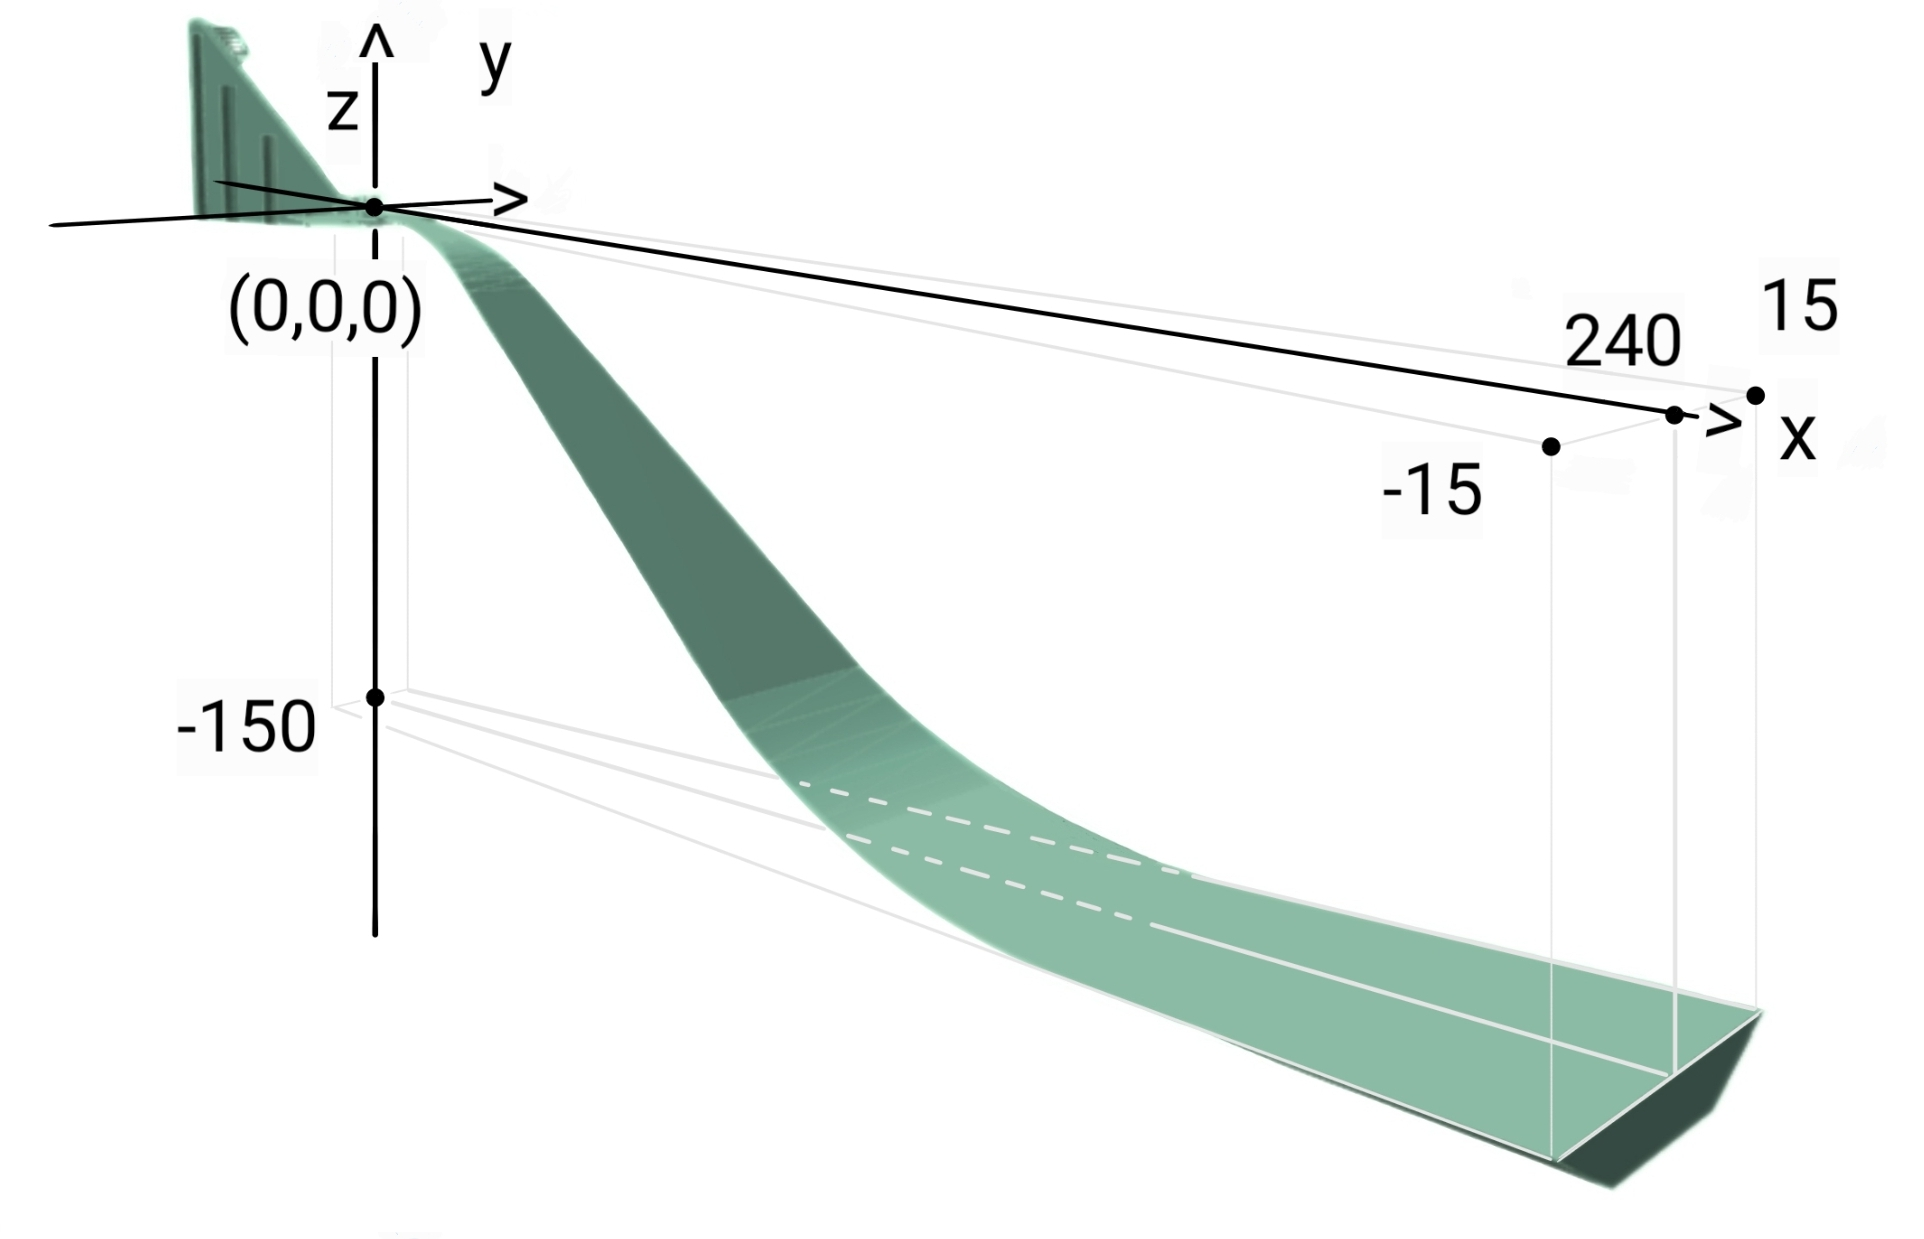
\includegraphics[width=\linewidth]{koncen_graf.jpg}
  \caption{3D model of Ski jump in Planica with added coordinates \cite{skisprungschanzen_letalnica, 3dmdb_skijumping_planica}}
  \Description{A model of ski jump in Planica, showing X, Y and Z axis}
  \label{fig:planica}
\end{figure}

\begin{figure}[h]
  \centering
  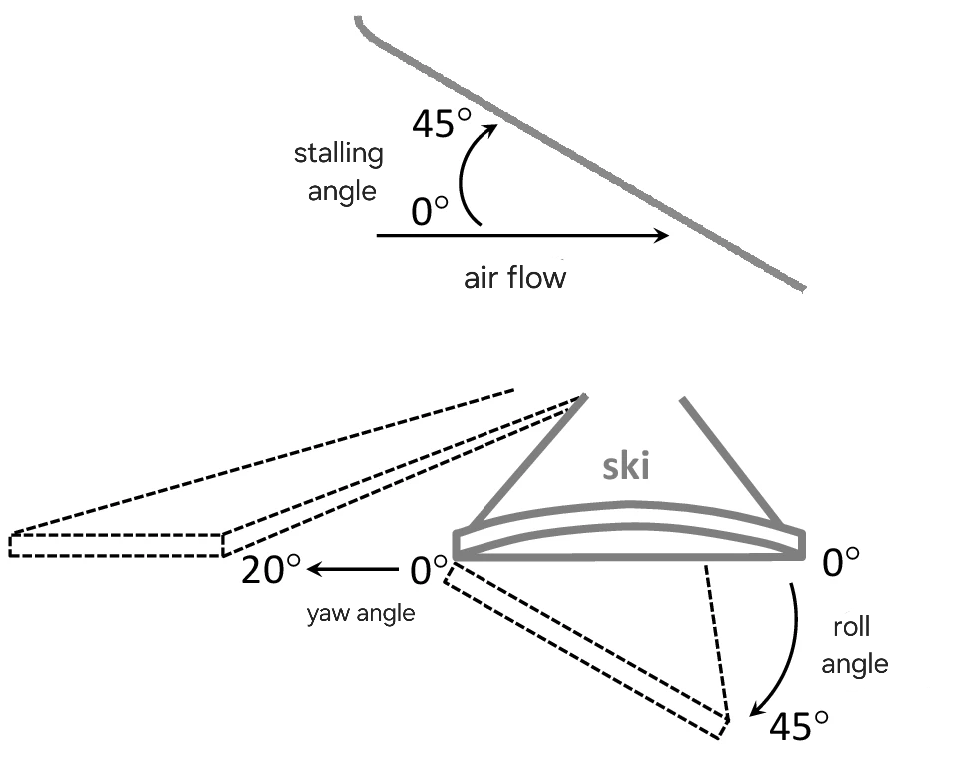
\includegraphics[width=\linewidth]{koti.png}
  \caption{Different angles affecting the jump}
  \Description{Representation of stalling, yaw and roll angles next to a ski jumper's skis}
  \label{fig:koti}
\end{figure}

The wind features are as follows:
\begin{description}
    \item [WindTime] - time of the wind measurement in the same format as the Time column itself. Since wind measurements are recorded less often, the wind values are applied to the most recent jump measurement and then just repeated until a new wind measurement is available. Since the wind is represented by a nonlinear function, it would be hard to capture its movements with interpolation, so we decided to drop this column.
    \item [WindName] - name of the sensor (Wi for $i = 1,\ldots,12$)
    \item [WindSpeed] - resulting speed of the wind in km/h 
    \item [WindSpeedTangent] - speed of the wind tangent measured along the x axis (hill direction) in km/h
    \item [WindTurbulence] - vertical speed of the wind turbulence in km/h
    \item [WindSpeedCleanTan] - wind speed tangent with\\
     turbulence removed in km/h
    \item [WindSpeedCross] - speed of the wind measurement along the y axis across the hill in km/h
\end{description}

There are $12$ wind sensors spread across the ski jump hill. To help with
the analysis, we separated the jump section of the hill into $3$ zones. The first zone
contains wind sensors $1$ to $4$, the second zone contains sensors $5$ to $8$, and the third zone contains sensors $9$ to $12$ \cite{SkiJumping_Book}. 

During processing, we also removed some ski jumps that were incomplete or had corrupted data, so the
final dataset contained around $200$ ski jumps.

\section{Methodology}\label{sec:method}
This section describes our research methodology. We first present different variations of the SSM that we tested for the ski jump simulation, followed by describing our model and how it predicts the jumps. Finally, we present the description of our ski jump animation app.

\subsection{Different modeling approaches}

%pač to je tko idejno, recimo k si probala različne stvari, kaj kako dela, sej 
%ne vem če sm prou napisala, če nism lahko popraviš, sam tko se je slišal fensi
%no tuki se mi zdi da na kratko sam kaj je blo probano polpa natancno kar mava 
%zdej v naslednjem subsectionu

In addition to pure SSM, we considered different approaches for modeling ski jumps that included classical physics-based models, but the data are not sufficient to accurately capture all the forces acting on the jumper.
We also tried a hybrid approach that combined SSM and Physics-informed Neural Networks (PINNs \cite{StatQuest_NN_YouTube}), where
the SSM would provide a baseline prediction and the PINN would learn to correct any discrepancies, taking into account physical properties of the system, such as the mass of the pilot, the properties of the wind, and gravitational force \cite{Cai2021_PINN_FluidMechanics}. 
These parameters are included in the equations of motion and added to the total loss function. 
So, the model prefers solutions that are consistent with the laws of physics. This
turned out to be less effective than a pure SSM approach, but the reason exceeds the purpose of this paper. More about errors and models' comparison is given in Section \ref{sec:error}.


\subsection{Ski jump prediction model}

In order to fit our data to the SSM, we stored the data in each file in three vectors.
The main vector contains states or state variables of the system, which in our case are the
X, Y, and Z coordinates, jumper velocities for each of the directions, resulting speed, and all angles (opening, stalling, roll, and yaw) \cite{CERN_SkiJump_Physics}.

The observation vector contains the measured outputs of the
system, which in our case are the X, Y, and Z coordinates and
height above ground. The controls contain the external inputs to
the system, which in our case are the wind measurements from
all the sensors for each of the features (speed, tangent, cross and
turbulence) that are then averaged over each zone combined with
all the angles (resulting speed, opening, and for both left and right
ski the roll, yaw and stall angles).



We then used ridge regression to estimate the matrices $A$, $B$, $C$
and $D$ of the SSM, as shown in Figure \ref{fig:matrices}, where we minimized the
computed values from the current and previous values and the next
time-stamped values. The next value is simulated through matrix
multiplication with state, controls and observations vectors. For
our simulation we specifically focus on $A$ and $B$ matrices, since
we want to predict the next state from the current state and the
current control. The $C$ and $D$ matrices are used to predict the next
observation, but since we are interested in the trajectory, we don’t
use them for simulation. Thus, matrix $A$ computes the next state
from the current state, $B$ computes the next state from the current
control, $C$ computes the next observation from the current state,
and $D$ computes the next observation from the current control. We
then combine the predictions for next state and the next control to
get the next simulated value, which allows us to then use recursion
to get the full simulated jump. This allows us to predict the jump
trajectory based on the environmental conditions and the starting
state of the jumper \cite{SSM_YouTube}. 

\begin{figure}[h]
  \centering
  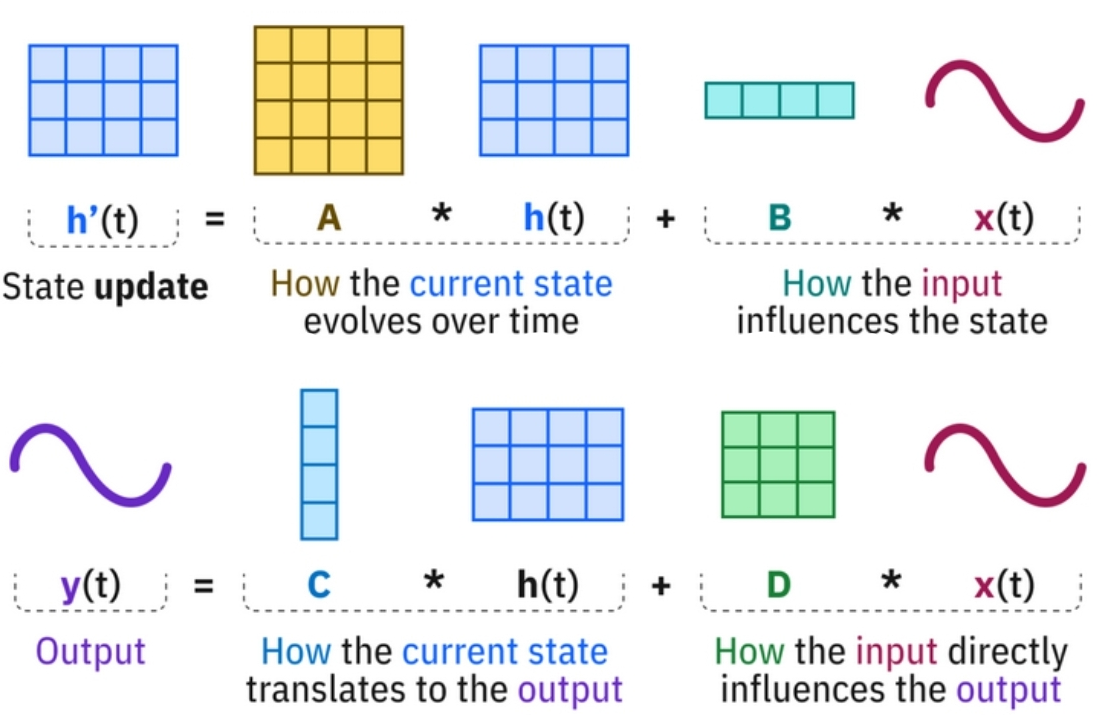
\includegraphics[width=\linewidth]{shema_matrik.png}
  \caption{Schema of SSM matrices \cite{bergmann2025state_space_model}}
  \Description{Two equations with pictures, showing what each $A$, $B$, $C$, and $D$ matrices mean in SSM}
  \label{fig:matrices}
\end{figure}

\subsection{Average file starter}

Since the goal is to have an interactive application where users can
adjust the wind conditions and angles and observe the impact on
the jump, we needed to find a way to start the simulation with the
initial state of the jumper, that wouldn't be too specific to a single
jump. We created an average file, where the values for each column
are averaged over all the jumps in the dataset. Since the flights are
of different lengths and measured at different time stamps, we first
had to interpolate the jumps to get the average number of time
stamps and the average length of the jump.

We then used the first row of the average file as the starting
point for the simulation, which contains the average values for
all the features at the take-off point. This allows the simulation to
start with realistic initial conditions that are representative of the
average jump in the dataset. And in case there is no external input
from the user for a certain wind or angle, the simulation will just use
the average values from the file as the default input, which allows
the user to see a realistic jump trajectory even without adjusting
the inputs.

We then calculated the matrices $A$ and $B$ using the same process
as before on all of the jumps in the dataset. This allowed us to connect them with the app, so the user gets a realistic jump trajectory
based on his inputs.

\subsection{Ski jump animation app}

To make our results accessible beyond the research setting, we developed an interactive web application using Shiny for Python \cite{shiny_python}. The application serves as a front-end to the trained state-space model and allows users to explore ski jump simulations under varying environmental conditions or just to observe different measured ski jumps. Firstly, through a set of input controls, users can adjust factors such as wind speed, wind directions, or different ski angles, and the application instantly updates the predicted jump trajectory.
Secondly, users can simply explore random jumps from the provided dataset or upload their own CSV file of measured jumps, as long as it includes the columns described in Section \ref{sec:processing}.

The application presents the results as an animated visualization of the ski jump, 
showing the full trajectory and the final distance. In this way, the application functions both as an analytical tool, helping to test how different conditions affect performance, and as an educational resource that makes the mechanics of ski jumping easier to understand for a wider audience. It is available online. \footnote{\url{https://camlekn.shinyapps.io/ski-jump/}}

\section{Main results}\label{sec:results}
In this section, we present the results of our simulations. Firstly, we present a statistical comparison of all the models, followed by a precise analysis of our predictions.

\subsection{Models' error}\label{sec:error}
In order to evaluate different models, we first had to define a metric to
measure the prediction error. Since actual and simulated jumps are represented
with x, y, and z coordinates but are measured at different time stamps and can
contain a different number of measurements, we had to find a way to compare
them. Since time stamps represent the athlete's position on a coordinate system 
at different times, we decided the time information isn't as crucial as the 
position and consequently the distance of the jump. Which allowed us to compare
the actual and simulated jumps irrespective of the information about time.

We first tried to project the shorter trajectory on to the other one and
compute the distance between the original and the projection, but this method
turned out to be computationally expensive. So we decided to compute the
distance between the actual and the simulated jumps by interpolating both
jumps. The new measurements contain the start and end point and all the ones,
where x reaches a natural value. We then compute the error as the norm of the
difference between the two jumps. And after one of the jumps ends, we just add
the distance from the end of the shorter jump to the end of the longer jump to
the error. This way, we penalize the model for not being able to predict the
correct length of the jump, while still keeping the interpretability of the
error as the distance between the two jumps.

We then used a KFold cross-validation to evaluate the models. KFold is a method 
of splitting the dataset into $K$ subsets, or folds, and then train the model $K$ times,
each time using a different fold as a test set and the remaining folds as a training set.
Since we already had a very limited number of jumps, we used the leave-one-out 
cross-validation version of the algorithm, where $K$ is equal to the number of jumps 
in the dataset. This allows us to use as much data as possible for training while 
still providing a robust evaluation of the model's performance on unseen data.
We then computed the average error between the actual jump and the simulated jump 
for both the training set and the test set, as shown in Figure~\ref{fig:actual_vs_sim}. 
We also made a baseline evaluation of the error by comparing the actual jump to the
average jump from the average file. The error for both the trained and the test dataset 
is the same ($2.72$ m) since the average file is the same for both datasets.

At the end it turned out that the best model was the pure SSM with averaged wind
data over the zones, which with the leave-one-out algorithm achieved an average 
error of $1.32$ m on the training data and $1.37$ m on the test data. And when we use
starting point from the average file instead of the actual starting point of the 
jump, the error is $1.58$ m on the training data and $1.63$ m on the test data.
So we can interpret the error as: If we were to choose a random point on the simulated
path, then the athlete would be on average $1.63$ m away from the actual path of the jump.

This suggests that averaging the wind data over the zones helps to
reduce noise and improve the model's ability to generalize from the training data 
to unseen jumps.

\begin{figure}[h]
	\centering
	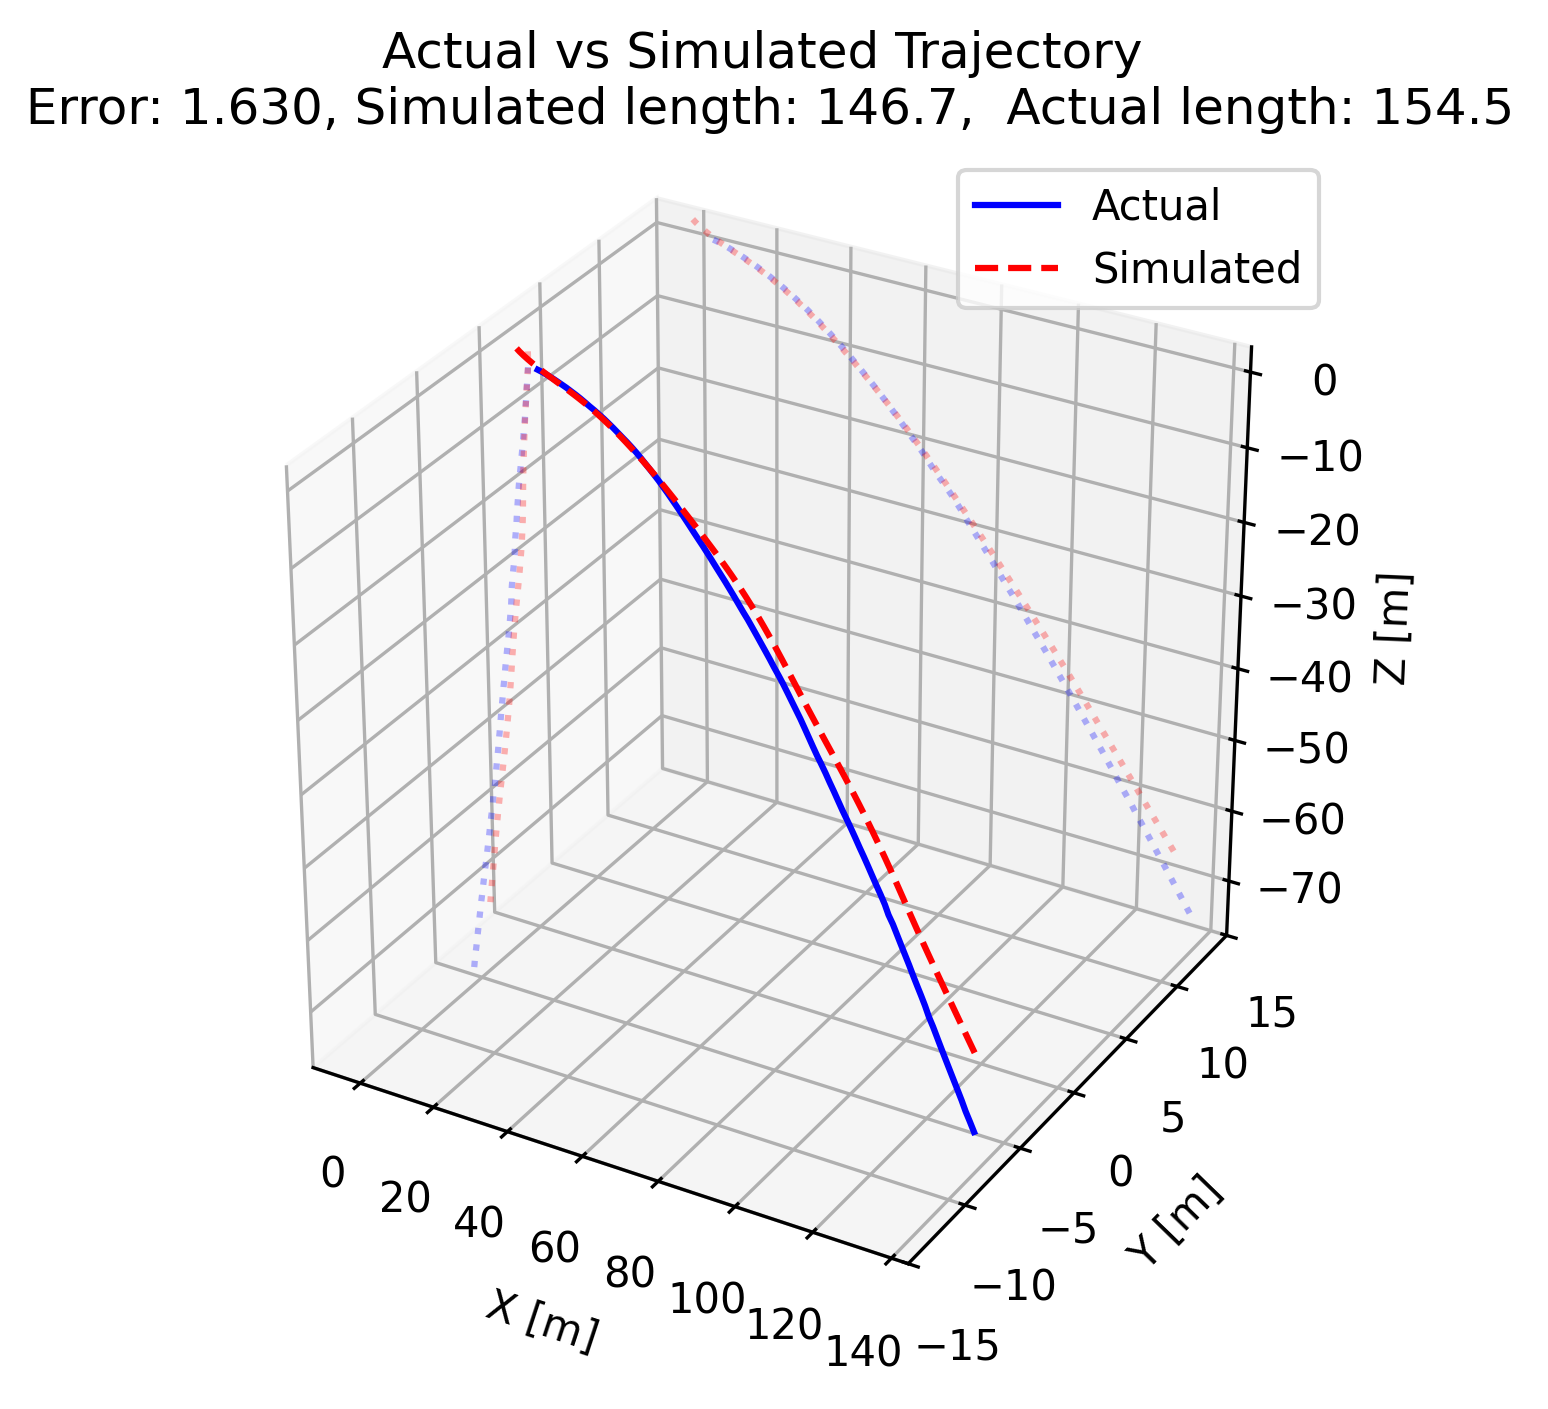
\includegraphics[width=\linewidth]{2SSM_flight_simulation123.png}
	\caption{Actual vs. simulated ski jump trajectory}
	\Description{A graph comparing an actual jump trajectory to the simulated one}
	\label{fig:actual_vs_sim}
\end{figure}

\subsection{Analysis of our model}

In the process of developing our ski jump prediction model, we evaluated several
variations to determine the most effective approach. We compared the
performance of a pure SSM with a hybrid model that combined SSM with PINN. The
pure SSM demonstrated superior predictive accuracy, probably due to its ability
to directly model the temporal dynamics of ski jumps without the added
complexity of PINNs.

We tested the impact of wind features on the model's performance by training
the models with the information of every wind sensor instead of averaging the wind
data over zones. However, this approach resulted in a higher prediction error 
(with the error measuring $1.62$ m on the training data and $1.82$ m on the test data),
likely due to the increased noise and variability in the data from the individual
sensors, which may have made it more difficult for the model to learn the underlying
patterns in the data. 

Wind is a critical factor in ski jumping, so we attempted to capture its
nonlinear effects by including columns for the squared wind features. However,
we found that adding these squared terms did not help with the prediction, and 
in fact, it increased the error (with the error measuring $1.33$ m on training 
data and $1.43$ m on test data). This suggests that the relationship between wind
and jump trajectory may not be well captured by simple polynomial terms.

Here we present all the results of the different models in Table~\ref{tab:models_comparison}.

\begin{table}[h]
	\centering
	\begin{tabular}{p{4.0cm}cc}
		\toprule
		Model & Training Error & Test Error \\
		\midrule
		SSM with averaged wind data & $1.32$ m & $1.37$ m \\
		SSM with averaged wind data and average starting point & $1.58$ m & $1.63$ m \\
		SSM with individual wind sensor data & $1.62$ m & $1.82$ m \\
		SSM with averaged wind data and squared wind features & $1.33$ m & $1.43$ m \\
		\bottomrule
	\end{tabular}
	\caption{Comparison of different models based on training and test error}
	\label{tab:models_comparison}
\end{table}

%\vspace{-0.7cm}

Since the simulation still requires numerous inputs, we made it interactive,
allowing users to adjust the wind conditions and observe their impact on the
jump. In the ski jumping app, users can manipulate sliders to set the wind
speed, wind tangent, wind cross, and wind turbulence for each of the three
zones. As a result, the wind loses its original movement function in the
simulation. All other inputs are set to the average values computed from the
dataset.



\subsection{Analysis of model's parameters}
To better understand the model's behavior, we analyzed the parameters of the 
matrices $A$ and $B$. 

Matrix $A$ suggests that the SSM is capturing two different physical regimes: 
slow kinematics and fast aerodynamic control. The strongest values are the 
diagonal terms for X, Y, and Z, which show that position depends overwhelmingly 
on its previous state. By contrast, posture variables are more reactive than 
persistent, especially Opening Angle, Roll, and Yaw, indicating active correction 
during the jump. The strongest non-diagonal dependency is $v_y$ $\rightarrow$  Roll Left ($0.302$), 
followed by $v_y$ $\rightarrow$ Roll Right ($0.233$), which implies that vertical motion is a major 
trigger for balance corrections. Another meaningful pattern is Opening Angle $\rightarrow$ Yaw 
Left/Right with opposite signs, suggesting that changing ski opening may also 
influence heading asymmetrically. In real-world terms, the jumper's path is smooth, 
but the body-ski system is continuously making small directional and balance adjustments 
to preserve lift and control.

Matrix $B$ indicates that environmental conditions are concentrated in the control layer 
of the system. The strongest dependencies are not on position, but on \texttt{Opening Angle}, 
\texttt{Roll}, \texttt{Yaw}, and \texttt{Stalling}, meaning the athlete mainly responds to 
disturbances by changing posture. The dominant external source is a variable
\texttt{landing\_Turbulence}, which strongly pushes opening, roll, and stalling responses. 
This makes physical sense: wind or unstable air does not instantly move the jumper's whole 
trajectory, but first forces the body-ski system to react, and those reactions then propagate 
into flight behavior.

\section{Discussion}
\label{sec:discussion}

%mal razglabljas o vsem, torej mal povežeš skupi kar sva do zdej povedali in 
%predlagava kkšne možne izboljšave mogoče
%torej najprej kok dobr je najna stvar delala, kako sva bli omejeni (mogoče da nisva meli ful velik podatkov?) in kaj še lahko in bova izboljsali


This section examines the predictive performance of the trajectories, highlights the limitations of our current approach, and suggests directions for future improvements.

\subsection{Limitations}

Given the relatively small dataset of ski jumps, the main limitation of our model lies in the limited data available for training the model.
%The main limitation of our project is the relatively small number of ski jumps available to train the model. 
After preprocessing, the dataset contained only about $200$ jumps, which may limit the SSM's ability to represent the full range of trajectory variations under different circumstances. As a result, the model may struggle to accurately predict jumps under novel or extreme conditions.

Furthermore, the dataset lacks detailed information, or any information at all, 
about individual jumpers, such as body weight, sex, or other physiological characteristics that are known to influence jump performance. Incorporating these variables could improve model accuracy and provide more personalized predictions \cite{muller2008performance}. 

Lastly, due to limited computing power, only one CPU was available, restricting the use of possible better models. To address these challenges, using cloud-based resources could help run larger models and improve the prediction of trajectories.

\subsection{Future work and potential improvements}

Although the current approach shows promise, there are several avenues for
future improvements. Some of which we are working on at the time of writing
this paper.

Currently, we are working on improving the sliders’ functions on the web application. Since the wind
data determined by the user is static throughout the jump, this adds a lot of
generalization. In reality, wind conditions can change rapidly during a jump.
So we would like to add additional controls to the app that would allow the
user to define how the wind changes during the jump. They could choose whether
the wind would gain or lose a certain feature (such as speed or turbulence)
during the jump.

Expanding the dataset to include more jumps and additional contextual
information about individual jumpers could improve the accuracy of the model.
We could try to generate more data by using data augmentation techniques, such
as adding noise to the wind measurements or slightly modifying the angles. We
could also try to find the nonlinear movements of the wind and interpolating
the wind measurements by their original time stamps to better capture the wind
dynamics.


\section{Conclusion}\label{sec:conclusion}

This paper presents a method for predicting ski jump trajectories based on environmental conditions. By incorporating external factors into the modeling framework and applying least squares estimation, we demonstrated that the model is capable of capturing the dynamics of ski jumps and producing realistic trajectory predictions. In addition, we developed an interactive application that makes the results accessible to a broader audience through simulations and animations of predicted jumps. Although the current model is limited by the size of the dataset and the absence of certain athlete-specific variables, the results show that state-space models are a promising tool for analyzing ski jumping performance.

\section{Acknowledgments}
This work was supported by the Slovenian Research and Innovation Agency(ARIS) via the Research Program Knowledge Technologies(grant P2-0103) and the European Commission through the Horizon Europe projects SLAIF (grant 101254461), ELIAS (grant 101120237), and HumAlne (grant 101120218). We would like to thank Smučarska Zveza Slovenije (Ski Association of Slovenia) for providing the ski jump data.
%%
%% The next two lines define the bibliography style to be used, and
%% the bibliography file.
% 

\appendix



\printbibliography
\end{document}
\endinput